\documentclass[11pt,a4paper]{article} 
\usepackage[danish]{babel}
\usepackage[utf8]{inputenc}
\usepackage{graphicx}

\begin{document}

\section{Synopsis}
Faget “Introduktion til computergrafik” gav et indblik i 3D computergrafik, dette projekt arbejde videre med computergrafik, hvor faget slap. Projektet omhandler hvordan dobbeltkrumme flader beskrevet ved polynomier skyggerlægges. Skyggelægning er vigtigt del af computergrafik fordi skygger opstår alle steder i naturen, for at et 3D billede kan se naturligt ud bliver skygger nødt til at være en del af billedet. Projektet vil kigge på forskellige skyggerlæggnings metoder, sammenligne disse og lave en implementering af nogle af dem.

\section{Afgrænsning}
Dette projekt vil behandle skyggelægnings algoritmerne med fokus på to mest anvendte: shadow map og shadow volumen. De to skyggelæggninges algoritmer vil blive behandlet, og der vil blive taget stilling til og forklaret mulighederne for hvordan man på en enkelt måde kan opnå væsentlige bedre resultater med de 2 algoritmer. Især fordele og ulemper ved de to algoritmer vil blive behandlet. For shadow map vil et spotlight blive brugt som lyskilde mens det for shadow volumen vil blive brugt en point light lyskilde. Der vil kun blive brugt en lyskilde pr. algoritme men implantationen vil være så general at det nemt vil kunne udvides med flere lyskilder. Den teoretisk på hastigheden af algoritmen,  vil ikke være i fokus da jeg ikke bestræber mig på at implementere algoritmerne på den mest effektive måde, køretiden for algoritmerne vil blive testet..

Produktet af denne opgave vil være et bachelorprojekt rapporten der vil beskrive teorien bag de to algoritmer samt et program, der kan anvende de to skyggelæggninges algoritmer, og vil blive implementeret i C, openGL og glsl. Der vil kun blive arbejdet med point light sources, hvor alt lys fra lyskilden kommer af et enkelt punkt.
\section{Tidsplan}

Herunder tidsplanen for projektet.

\begin{figure}[ht!]
\centering
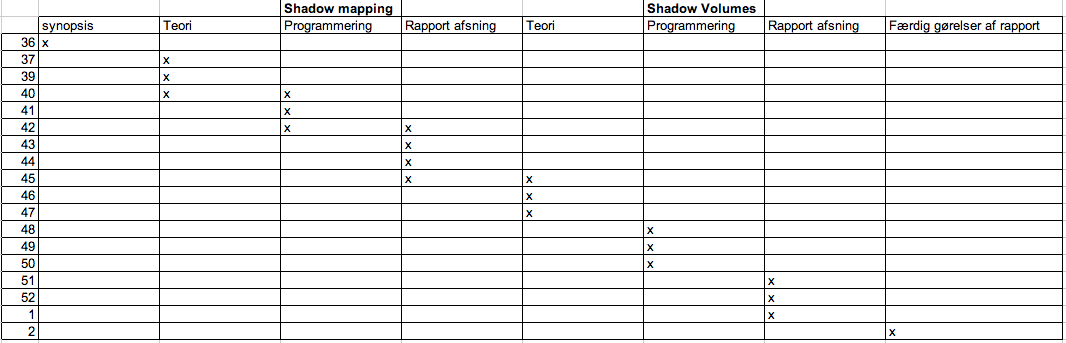
\includegraphics[width=140mm]{tid.png}
\caption{Tidsplan}
\label{S4}
\end{figure}




\end{document}